\chapter{Definice formátu animace}

V této kapitole je popsán postup a~algoritmus vytváření animace. Jedná se o~zjednodušený algoritmus, který v podobné podobě používá například formát APNG\cite{apngFrames}. 


\section{Popis formátu animace}

Nástroj pro generování animace má za úkol přeformátovat vstupní animaci z~různých zdrojů (GIF, .mp4, .jpg) do tohoto formátu. Celý princip je založený na~tom, že se mezi jednotlivými snímky mění pouze část vykreslovaného pole (viz obrázek \ref{fig:algdiffs}). My si budeme ukládat informace o~tomto fragmentu a~jeho obsah. Tyto data poté uložíme do dvou souborů, podle kterých se bude řídit přehrávání. V~následujícím textu si projdeme všechny úkony, které algoritmus vytváří.

\subsection*{Snímky animace}

Jednotlivé fragmenty ze snímků budeme ukládat do jednoho velkého obrázku, který se bude po částech zase vykreslovat při přehrávání. Musíme zajistit, aby byly fragmenty vždy pouze jednou, abychom zajistili minimální možnou velikost dat. 


\section{Algoritmus zakódování z~dostupných formátů}
\label{section:algencode}

Tato sekce dokumentuje celý algoritmus výpočtu animace. Rozdělení tohoto algoritmu do tříd je podrobně popsáno u~návrhového modelu. 

\subsection{Inicializace}
Algoritmus na~vstupu dostane množinu snímků animace reprezentovanými maticí obrázků. První snímek slouží jako počáteční stav. 

\begin{figure}[h]
\centering

\includegraphics[width=1\textwidth]{figures/alg-frames.png}
\caption{Snímky ukázkové animace}
\label{fig:algframes}
\end{figure}

Pro lepší porozumění použijeme animaci západu slunce, animace má pouze 4 snímky kvůli jednoduchosti, ale dokážeme na ní předvést veškeré operace, které algoritmus provádí.


\subsection{Rozdíly mezi snímky animace}
\label{section:algdiffsformat}

Algoritmus má tedy načtené snímky animace. Nyní prochází postupně snímek za snímkem a~sleduje změny oproti předchozímu snímku. Na následujícím obrázku vidíme změny znázorněny červeně.

\begin{figure}[h]
\centering

\includegraphics[width=1\textwidth]{figures/alg-diffs.png}
\caption{Rozdíly mezi snímky animace}
\label{fig:algdiffs}
\end{figure}


\subsection{Optimalizace rozdílů snímků}

Algoritmus zajišťuje, aby rozdíly mezi snímky se shlukly do větších bloků, kvůli ušetření režie následného přehrávání. Na následujícím obrázku lze vidět, že algoritmus dal dohromady paprsky slunce se samotným sluncem. Tyto jednotlivé části animace poskláda do jednoho velkého obrázku a~zapamatuje si pozici (obrázek \ref{fig:algdiffs}). 

\begin{figure}[h]
\centering

\includegraphics[width=1\textwidth]{figures/alg-simplify.png}
\caption{Optimalizace rozdílů snímků}
\label{fig:algsimplify}
\end{figure}
\FloatBarrier

\subsection{Zakódovaná animace}

Prvním souborem na výstupu je výsledná bitmapa, kterou program uloží ve formátu PNG (obrázek \ref{fig:algresult}). Informace o~průběhu animace a~nalezené jednotlivé rozdíly jsou pak uloženy v~druhém souboru.

\begin{figure}[h]
\centering

\includegraphics[height=200pt]{figures/alg-result.png}
\caption{Grafika odeslaná na výstup}
\label{fig:algresult}
\end{figure}


\section{Přehrávání}

Při přehrávání máme k~dispozici obrázek se všemi částmi animace (obrázek \ref{fig:algresult}) a~soubor s~meta informacemi. Tedy informacemi, kdy a~co se má zobrazit v~animaci. K~výše uvedenému obrázku například existuje soubor, který nese souřadnice co se má zobrazit v~aktuálním snímku (obrázek \ref{fig:algmetadata}).

Přehrávač potom postupně zobrazuje části obrázku podle daných informací. 

\begin{figure}[h]
\centering
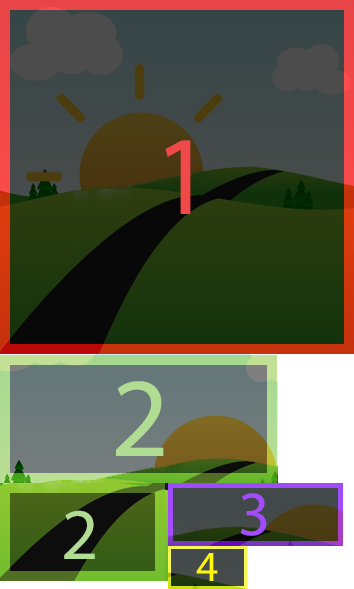
\includegraphics[height=200pt]{figures/alg-metadata.png}
\caption{Informace o~snímcích, které nese druhý soubor animace}
\label{fig:algmetadata}
\end{figure}


